\textit{Dancing With The Stars} (DWTS) combines judges' scores with audience voting to eliminate contestants weekly, yet the audience vote totals remain confidential. \cite{comap2026_problemC_pdf}
This creates a persistent tension between ``technical merit'' and ``popular support,'' further complicated by format changes across seasons (rank-based vs.\ percent-based aggregation, and the later Bottom-2 judges' save).
The provided dataset \cite{comap2026_problemC_data} spans 34 seasons with contestant attributes, weekly judges' scores, and realized eliminations, but it does not reveal audience votes---making fan preference a latent signal that must be inferred from outcomes.

\begin{figure}[H]
  \centering
  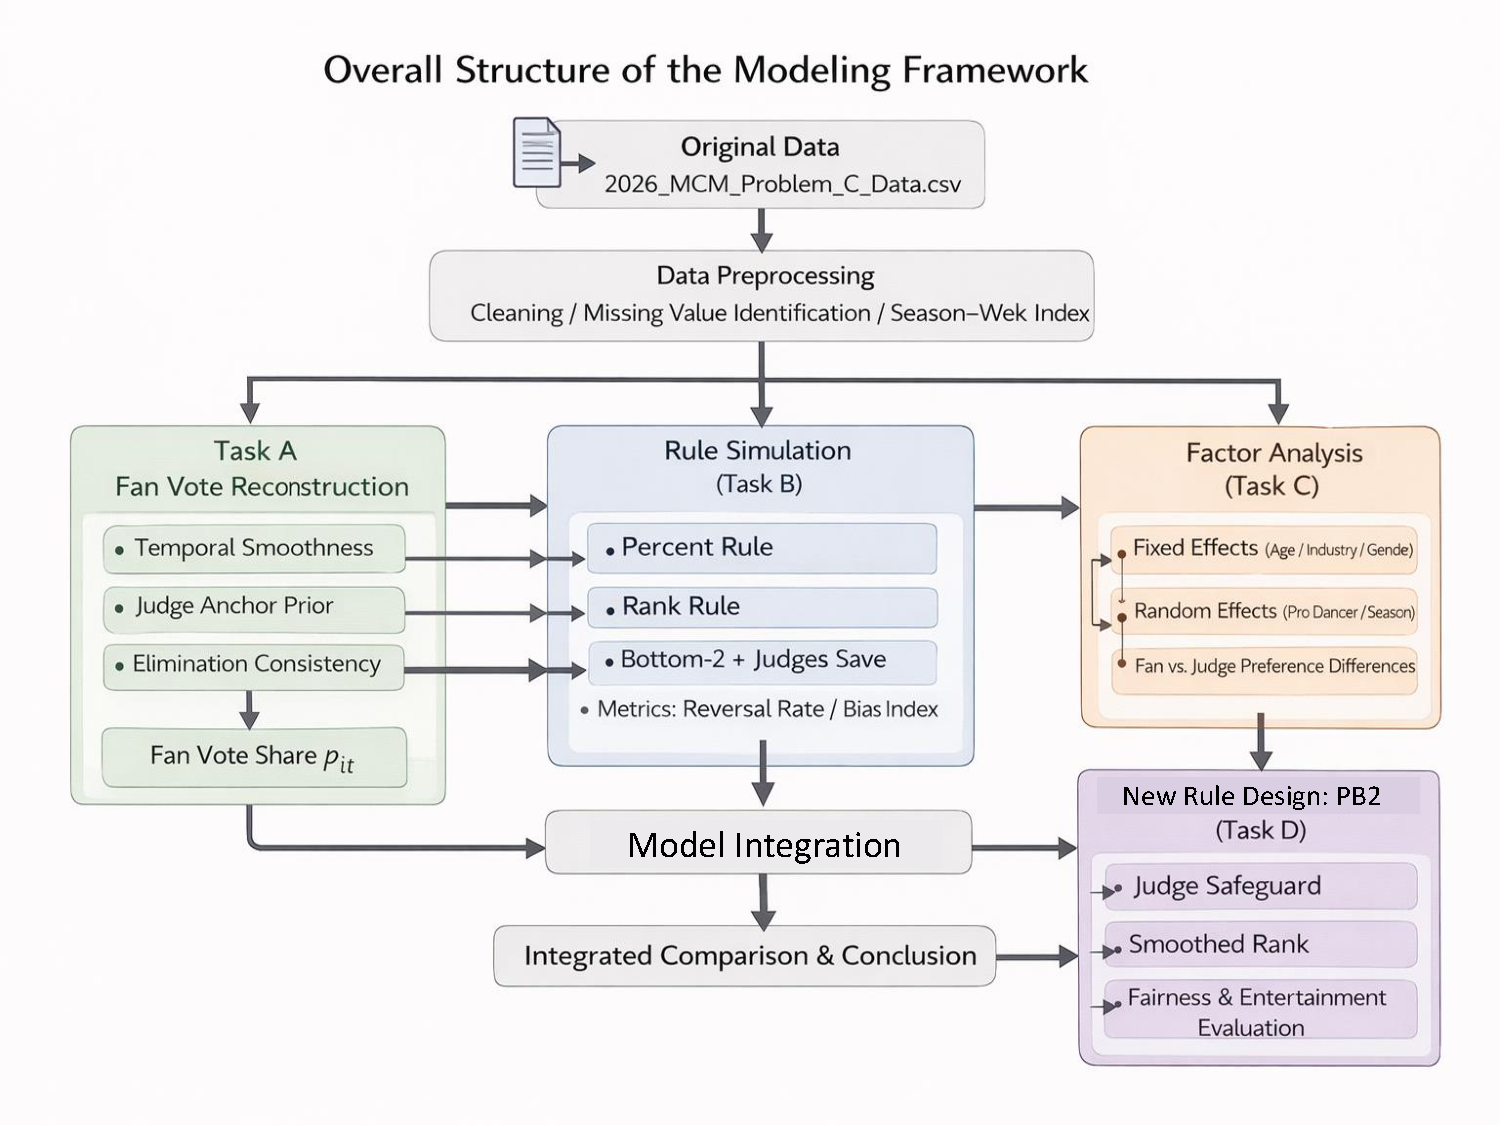
\includegraphics[width=0.65\linewidth]{output/fig/task3/overview.pdf}
  \caption{End-to-end workflow: infer latent fan support from observed eliminations, then use it to evaluate and redesign voting rules.}
  \label{fig:workflow_overview}
\end{figure}

\textbf{We model DWTS as a replayable inverse problem: infer latent fan support from observed eliminations, then use it to evaluate and redesign voting rules.}
(An end-to-end workflow summary is provided in the Summary Sheet; we keep the Introduction focused on motivation and contributions.)

\textbf{Our contributions are as follows.}
\begin{itemize}
  \item \textbf{Replay-ready data representation.}
  We build a canonical season-week-contestant panel with an explicit \texttt{active} set to ensure that all denominators and eligibility conditions match the show's mechanics (and that post-exit padding records do not contaminate comparisons).

  \item \textbf{Latent vote-share inference with uncertainty.}
  We infer weekly fan vote \emph{shares} by solving a constrained optimization problem whose feasibility encodes elimination consistency; slack handles exceptional weeks, and a smoothness prior selects stable explanations.
  The output includes both point estimates and uncertainty summaries (feasible ranges / sensitivity margins), supporting identifiability-aware interpretation.

  \item \textbf{Counterfactual rule evaluation via replay.}
  Using the inferred fan support, we replay eliminations under alternative aggregation schemes (rank vs.\ percent) and the incumbent Bottom-2 + judges' save mechanism, and quantify outcome divergence and robustness with replay-based metrics aligned to the show's decisions.

  \item \textbf{Mechanism analysis and transparent redesign (Task D2).}
  We fit interpretable statistical models to separate drivers of judges' scoring from fan preference (e.g., professional-dancer and celebrity-attribute effects), and propose \textit{Professional Bottom-2} (PB2): judges define the Bottom-2 risk set, while fan influence is applied only within that gate via a transparent blended score.
  PB2 is validated by replay-based stress tests (stability, controversial-case replays, and a unified bias test).
\end{itemize}

The remainder of the paper is organized as follows:
Section~2 formalizes tasks, assumptions, and notation;
Section~3 describes data processing and feature construction;
Sections~4--7 present vote inference, rule replay, mechanism analysis, and PB2 with robustness tests;
Section~8 concludes; and Section~9 provides a memo to management.
